\documentclass[11pt]{article}
\usepackage{fullpage}
\usepackage{amsthm}
\usepackage{amsmath}
\usepackage{amssymb}
\usepackage{graphicx}

\graphicspath{ {./imgs/} }

\setlength{\parindent}{0pt}

\title{Information and Coding Theory (CO349) - Information Theory}
\author{Michael Tsang}

\newtheorem{defn}{Definition}
\newtheorem{eg}{Example}
\newtheorem{theo}{Theorem}
\newtheorem{lem}{Lemma}

\begin{document}

\maketitle

\section{Simple Codes and Coding}
\subsection{Motivation: Information and Security}
\textbf{Side-Channel Attacks:}
In optimised encryption algorithms, properties of the secret key determine the execution time.
If it is the case that zeroes lead to longer times and ones shorter then we could predict that when the algorithm runs for a longer time, the secret key contains more zeroes. \\
How much information about the secret key is revealed?
\\ \\
\textbf{Differential Privacy:}
In large statistical databases an attacker can try to reveal information (de-anonymise) individuals.
Suppose there are three individuals under 25 with hair loss registred and two individuals are getting hair loss treatment in SW7.
Kim is on the database, is 21, and lives at 170 Queen's Gate. \\
How much information about individuals is revealed?

\subsection{Entropy}
\begin{defn}
  The \textbf{entropy} of a probability distribution $p$ is:
  \[ H(p) = - \sum p(x) \log_{2} (p(x)) \].
\end{defn}

\subsection{Revision: Logarithms}
\begin{defn}
  Logarithms are defined implicitly via the equation:
  \[ x = b^{\log_{b} (x)}\]
\end{defn}

Useful identities:
\[ \log_{b} (xy) = \log_{b} (x) + \log_{b} (y) \]

\[ \log_{b} (x^{n}) = n \log_{b} (x) \]

\[ \log_{b} (x) = \frac{\log_{a} (x)}{\log_{a} (b)} \]

\subsection{Messages and Strings}
\begin{defn}
  An \textbf{alphabet} is a finite set $S$; its members $s \in S$ are \textbf{symbols}.
\end{defn}

\begin{defn}
  A \textbf{message} (or string, or word) $m$ in the alphabet $S$ is a finite sequence of elements in $S$:
  \[ m = s_1 s_2 \ldots s_n \text{ with } s_i \in S, 1 \leq i \leq n \]
  The number $n \in \mathbb{N}$ is the length of $m$, $\lvert m \rvert = n$.
\end{defn}

\begin{defn}
  A \textbf{prefix} of $m$ is defined:
  \[ m \rvert_{k} = s_1 s_2 \ldots s_k \text{ with } k \leq n \]
\end{defn}

\subsection{Notation}
\begin{defn}
  A string of length zero is denoted $\epsilon$, with $\lvert \epsilon \rvert = 0$.
\end{defn}

\begin{defn}
  $S^n$ denotes the set of all strings of length $n$, and
  \[ S^* = S^0 \cup S^1 \cup S^2 \cup \ldots \]
\end{defn}

\begin{eg}
  With the alphabet $S = \mathbb{B} = \{ 0, 1 \}$, we can produce all binary messages of a certain length $n$.
  \[ \mathbb{B}^3 = \{ 000, 001, 010, 011, 100, 101, 110, 111 \} \]
\end{eg}

\subsection{Coding}
\begin{defn}
  Let $S$ and $T$ be two alphabets; a \textbf{code} $c$ is an injective function
  \[ c : S \rightarrow T^* \]
\end{defn}

\begin{defn}
  For each symbol $s \in S$, the string $ c(s) \in T^*$ is called the \textbf{codeword} for $s$; the set of all code words is also referred to as the \textbf{code}:
  \[ C = \{ c(s) \mid s \in S \} \]
\end{defn}

An example is Morse code:
\[ c : \{ A, \ldots, Z \} \rightarrow \{ \bullet, -,\odot \} \]

\subsection{Decoding}
\begin{defn}
  A code $c : S \rightarrow T^*$ is extended to $S^*$ as follows: given a string $s_1 s_2 \ldots s_n$ in $S^*$ we define:
  \[ c(s_1 s_2 \ldots s_n) = c(s1) c(s2) \ldots c(s_n) \]
\end{defn}

\begin{defn}
  A code $c : S \rightarrow T^*$ is \textbf{uniquely decodeable (UD)} if the extended code function $c : S^* \rightarrow T^*$ is injective.
\end{defn}

This means that every string in $T^*$ corresponds to at most one message in $S^*$.

\subsection{Prefix-Free}
\begin{defn}
  A code $c : S \rightarrow T^*$ is \textbf{prefix-free (PF)} if there is no pair of codewords $q = c(s)$ and $q' = c(s')$ such that:
  \[ q' = qr \text{ for some non-empty word } r \in T^* \]
\end{defn}

\begin{eg}
  Let $S = \{ w, x, y, z\}$ with $c : S \rightarrow \mathbb{B}^*$ defined by:
  \begin{align*}
    w &\mapsto 10 & x &\mapsto 01 & y &\mapsto 11 & z &\mapsto 011
  \end{align*}
  The code is not PF, and it is not UD either:
  \begin{align*}
    wxwy &\mapsto 10011011 & wzz &\mapsto 10011011
  \end{align*}
\end{eg}

\subsection{PF implies UD}
\begin{defn}
  If a code $c : S \rightarrow T^*$ is prefix-free then it is uniquely decodeable.
\end{defn}

\textbf{Proof:}
Given that a code $c$ is prefix-free, let us assume that it is not uniquely decodeable.
Then there is an $x = x_1 x_2 \ldots x_m$ and a $y = y_1 y_2 \ldots y_n$ such that $c(x) = c(y)$, where $c(x) = c(x_1) c(x_2) \ldots c(x_m)$ and $c(y) = c(y_1) c(y_2) \ldots c(y_n)$. \\

The prefixes must be the same $c(x) \rvert_{k} = c(y) \rvert_{k}$ for any $k$, but it might be that $\lvert c(x_1) \rvert \neq \lvert c(y_1) \rvert$.
Assume that $\lvert c(x_1) \rvert \leq \lvert c(y_1) \rvert$, and take $k = \lvert c(x_1) \rvert$ then $c(x) \rvert_{k} = c(x_1) = c(y_1) \rvert_{k}$.
Thus, $c(y_1) = c(x_1) r$ for some $r \in T^*$, this contradicts PF so it must be uniquely decodeable. \\

We repeat this to cover all of $c(x) = c(y)$.

\subsection{Strings and Codes in Trees}
If we concentrate on binary codes with $T = \mathbb{B}$, any codeword in $C$ can be seen as a finite path in a binary tree.
Moreover, the codewords in $C$ can be represented as the end-points of the corresponding paths: if a code $c$ is PF then none of its decendents can represent a codeword in $C$.

\begin{eg}
  The code $C = \{ 0, 10, 110, 111 \}$ is PF, its corresponding tree is shown in figure \ref{fig:treepath}.
  \begin{figure}[h!]
    \caption{Tree for the given code $C$.}
    \centering
    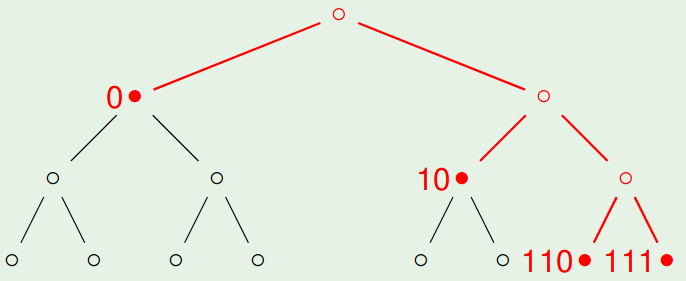
\includegraphics[width=\textwidth]{treepaths}
    \label{fig:treepath}
  \end{figure}
\end{eg}

\subsection{Parameters of a Code}
\begin{defn}
  Given a code $c: S \rightarrow T^*$, let $n_i$ denote the number of symbols $s \in S$ which are \textbf{decoded} by strings of length $i$:
  \[ n_i = \lvert \{ s \in S \mid \lvert c(s) \rvert = i \} \rvert = \lvert \{ s \in S \mid c(s) \in T^i \} \rvert \]
\end{defn}

We refer to $n_1, n_2, \ldots, n_M$ as parameters of $c$, where $M$ is the maximal length of a codeword.

\begin{defn}
  The number of all \textbf{potential codewords} of length $i$ is given by:
  \[ b^i = \lvert T^i \rvert \]
  In particular: 
  \[ b = \lvert T \rvert = b^1 \]
\end{defn}

\begin{defn}
  The \textbf{filling rate} is the fraction of possible codewords of length $i$ actually used by a code is:
  \[ \frac{n_i}{b^i} \]
\end{defn}

\subsection{Kraft-McMillan Number}
\begin{defn}
  Given a code $c : S \rightarrow T^*$ with parameters $n_1, n_2, \ldots, n_M$, the \textbf{Kraft-McMillan number} of $c$ is:
  \[ K = \sum_{i = 1}^{M} \frac{n_i}{b^i} = \frac{n_1}{b} + \frac{n_2}{b^2} + \ldots + \frac{n_M}{b^M} \]
\end{defn}

\begin{eg}
  Considering a binary code $C = \{ 0, 10, 110, 111 \}$:
  \[ K = \frac{1}{2} + \frac{1}{4} + \frac{2}{8} = \frac{8}{8} = 1 \]
\end{eg}

\subsection{Existence of PF Codes}
\begin{theo}
  Given an alphabet $T$ with $\lvert T \rvert = b$ and parameters $n_1, n_2, \ldots, n_M \in \mathbb{N}$, if $K \leq 1$ then there exists a PF $b$-ary code $c : S \rightarrow T^*$ with these parameters.
\end{theo}

That is, there is a PF $b$-ary code with $n_1$ codewords of length $1$, $n_2$ codewords of length $2$, \ldots, $n_M$ codewords of length $M$.
In fact, if $K < 1$ then there is a more optimal PF code. \\

\textbf{Proof:}
Any partial sum of the one defining $K$ also fulfills $\sum_{i} \frac{n_i}{b^i} \leq 1$.
e.g.\ $\frac{n_1}{b^1} \leq 1$, $\frac{n_2}{b^2} \leq 1$, etc.

This implies:
\begin{align*}
  n_1 &\leq b & n_2 &\leq b(b^1 - n_1) & n_3 \leq b(b^3 - n_1b^1 - n_2) & &\text{etc \ldots}
\end{align*}

or in general:
\[ n_i \leq b(b^{i - 1} - n_1b^{i - 2} - n_2b^{i - 3} - \ldots - n_{i - 1}) \]

With codeword length $1$, since $n_1 \leq b^i$, we can choose any of them, $b - n_1$ words of length 1 remain as prefixes for words of length $2, 3, \ldots$

With codeword length $2$, there are $b^2$ codewords of length 2 but $b^1n_1$ are unavailable so $b^2 - b^1n_1$ are left.
However we have $n_2 \leq b(b - n_1)$ so we can make our choices, leaving $b^2 - n_1b - n_2$ prefixes of length 2 left.

With codeword length $i$, there are always $b^{i - 1} - n_1b^{i - 2} - n_2b^{i-3} - \ldots - n_{i - 1}$ prefixes of length $i - 1$ left, and from $K \leq 1$ we have:
\[ n_i \leq b(b^{i - 1} - n_1b^{i - 2} - n_2b^{i - 3} - \ldots - n_{i - 1}) \]

That is, we can choose enough codewords $n_i$ of length $i$ and enough remain.

\subsection{Encoding Strings}
\begin{defn}
  Consider a code $c : S \rightarrow T^*$ with parameters $n_1, n_2, \ldots, n_M$.
  Let $q_r(i)$ be the number of strings of length $r$ in $S^*$ encoded in a string of length $i$ in $T^*$.
\end{defn}

\begin{eg}
  Let $n_1 = 2, n_2 = 3$, what is $q_2(i)$?

  Since $x = x_1x_2 \in S^2$, then $c(x) \in T$ has lengths $2, 3, \text{ or } 4$.
  This is because $x_1, x_2 = 1 \text{ or } 2$ from the parameters.

  For $\lvert c(x_1x_2) \rvert = 2$: then $q_2(2) = n_1 \times n_1 = 2 \times 2 = 4$.

  For $\lvert c(x_1x_2) \rvert = 3$: then $q_2(3) = n_1 \times n_2 + n_2 \times n_1 = 2 \times 3 + 3 \times 2 = 12$.

  For $\lvert c(x_1x_2) \rvert = 4$: then $q_2(4) = n_2 \times n_2 = 3 \times 3 = 9$.
\end{eg}

\subsection{Generating Functions}
Generating functions are an important tool for investigating sequences, e.g.\ enumerations of combinatorial objects.

\begin{defn}
  For a sequence of numbers $q(1), q(2), q(3), \ldots$ the \textbf{generating function} $Q(x)$ is given as a polynomial (formal power series) in the unknown variable x:
  \[
    Q(x) = q(1)x + q(2)x^2 + q(3)x^3 + \ldots 
  \]

  For a code $c : S -> T^*$, we consider for $1 \leq i \leq rM$:
  \[
    q_r(i) = \lvert \{ \lvert c(s) \rvert = i \mid \lvert s \rvert = r \} \rvert
  \]

  and the generating function: 

  \[
    Q_r(x) = q_r(1)x + q_r(2)x^2 + q_r(3)x^3 + \ldots + q_r(rM)x^{rM}
  \]
\end{defn}

\subsection{Counting Principle (CP)}
\begin{theo}
  Given a UD code $c : S \rightarrow T^*$ with $\lvert c(s) \rvert \leq M$ for all $s \in S$ with generating function $Q_r(x)$ then for all $r \geq 1$:
  \[
    Q_r(x) = Q_1(x)^r
  \]
\end{theo}

\begin{eg}
  Following the previous example where $n_1 = 2, n_2 = 3$, what is the relationship between $Q_1$ and $Q_2$?

  It is clear that $q_1(1) = n_1 = 2$ and $q_1(2) = n_2 = 3$.
  We therefore have that:
  \begin{align*}
    Q_1(x) &= 2x + 3x^2 & Q_2(x) &= 4x^2 + 12x^3 + 9x^4
  \end{align*}
  and thus can see that:
  \[
    (Q_1(x))^2 = Q_2(x)
  \]
\end{eg}

\subsection{Kraft-McMillan Number for UD Codes}
\begin{theo}
  If there exists a UD code $c : S \rightarrow T^*$ with parameters $n_1, n_2, \ldots, n_M$ then $K \leq 1$.

  \[
    \exists UD \implies K \leq 1 \implies \exists PF \text{ and } PF \implies UD
  \]
\end{theo}

Then the following are equivalent for codes $c : S \rightarrow T^*$:
\begin{itemize}
  \item There exists a UD code with parameters $n_1, n_2, \ldots, n_M$.
  \item It holds that $K \leq 1$ for parameters $n_1, n_2, \ldots, n_M$.
  \item There exists a PF code with parameters $n_1, n_2, \ldots, n_M$.
\end{itemize}

\section{Probability}
Probability theory is concerned with quantifying or measuring the chances that certain events can happen.

We consider an event space, i.e.\ a finite set $\Omega$ and a set $\mathcal{B} \subseteq \mathcal{P}(\Omega)$ of measureable sets in $\Omega$ which form a Boolean algebra.
For finite sets we can use the power set $\mathcal{B} = \mathcal{P}(\Omega)$.

Probabilities are assigned via a \textbf{measure}, i.e.\ a function $Pr : \mathcal{B} \rightarrow \mathbb{R}$ or $m : \mathcal{B} \rightarrow \mathbb{R}$.

\subsection{Finite Probability Spaces}
Consider finite measureable spaces $(\Omega, \mathcal{B})$ with $\lvert \Omega \rvert = n$.

\begin{defn}
  A probability measure $Pr : \mathcal{B}$ on $(\Omega, \mathcal{B})$ has to fulfil:
  \begin{itemize}
    \item $Pr(\Omega) = 1$.
    \item $0 \leq Pr(A) \leq 1$ for all $A \in \mathcal{B}$.
    \item $Pr(A \cup B) = Pr(A) + Pr(B)$ for $A \cap B = \emptyset$.
  \end{itemize}
\end{defn}

Some further rules:
\begin{itemize}
  \item $Pr(\emptyset) = 0$.
  \item $Pr(\overline{A}) = 1 - Pr(A)$.
  \item $Pr(A \cup B) = Pr(A) + Pr(B) - Pr(A \cap B)$.
\end{itemize}

\subsection{Random Distributions}
For finite measureable spaces $(\Omega, \mathcal{B}, Pr)$ with $\lvert \Omega \rvert = n$, we can define a probability measure via atoms in $\omega \in \Omega$.

\begin{defn}
  A probability distribution is a function $\textbf{p} : \Omega \rightarrow [0, 1]$, with:
  \[
    \sum_{\omega \in \Omega} \textbf{p}(\omega) = 1
  \]
\end{defn}

If we enumerate the elements in $\Omega = \{\omega_1, \omega_2, \ldots, \omega_n \}$ in some arbitrary way, we can also represent $\textbf{p}$ by a row vector in $\mathbb{R}^n$:
\[
  \textbf{p} = (\textbf{p}(\omega_1), \textbf{p}(\omega_2), \ldots, \textbf{p}(\omega_n))
\]

\subsection{Random Variables} 
\[
  Pr(A) = \sum_{\omega \in A} \textbf{p}(\omega)
\]

\begin{defn}
  A \textbf{random variable} is a function $X : \omega \rightarrow \mathbb{R}$.
\end{defn}

\subsection{Moments in Probability}
\[
  \textbf{E}(X) = \sum_{\omega \in \Omega} \textbf{p}(\omega)X(\omega) = \sum_i \textbf{p}_i \textbf{X}_i = \mu_X
\]

\begin{align*}
  \textbf{E}(X + Y) &= \textbf{E(X)} + \textbf{E}(Y) & \textbf{E}(\alpha X) & \alpha \textbf{E}(X)
\end{align*}

\[
  Var(X) = \textbf{E}((X - \textbf{E}(X)))^2 = \textbf{E}(X^2) - (\textbf{E}(X))^2 = \sigma_X^2
\]

\subsection{Bayes Theorem and Independence}
Given two subsets $A$ and $B$ in a probability space $(\Omega, \mathcal{B}, Pr)$, the conditional probability of $A$ given that $B$ has happened is:

\[
  Pr_B(A) = Pr(A \mid B) = \frac{Pr(A \cup B)}{Pr(B)}
\]

Bayes Theorem states:
\[
  Pr_A(B) = \frac{Pr_B(A)Pr(B)}{Pr(A)} = \frac{Pr(A \mid B)Pr(B)}{Pr(A)} = Pr(A \mid B)
\]

$A$ and $B$ are independent if:
\[
  Pr(B) = Pr(B \mid A) = \frac{Pr(A \cup B)}{Pr(A)}
\]
or  
\[
  Pr(A \cup B) = Pr(A)Pr(B)
\]

\subsection{Products and Probability}
Given two probability spaces $(\Omega_1, Pr_1)$ and $(\Omega_2, Pr_2)$, to keep things simple use $\mathcal{B_i} = \mathcal{P}(\Omega_i)$, we can define a probability $Pr$ on the cartesian product $\Omega = \Omega_1 \times \Omega_2$ via:
\[
  Pr(\langle \omega_1, \omega_2 \rangle) = Pr_1(\omega_1)Pr_2(\omega_2)
\]

If $Pr_1$ and $Pr_2$ correspond to probability distributions $\textbf{p}_1$ and $\textbf{p}_2$, and $\textbf{p}$ to $Pr$ then $\textbf{p} = \textbf{p}_1 \otimes \textbf{p}_2$, the \textbf{tensor product}.

Not all distributions on $\Omega_1 \times \Omega_2$ are a product.

\subsection{Tensor/Kronecker Product}
Given a $n \times m$ matrix $\textbf{A}$ and a $k \times l$ matrix $\textbf{B}$:
\begin{align*}
  \textbf{A} &=
  \begin{pmatrix}
    a_{11} & \ldots & a_{1m} \\
    \dots & \ddots & \dots \\
    a_{n1} & \ldots & a_{nm}
  \end{pmatrix}
  &
  \textbf{B} &=
  \begin{pmatrix}
    b_{11} & \ldots & b_{1l} \\
    \dots & \ddots & \dots \\
    b_{k1} & \ldots & b_{kl}
  \end{pmatrix}
\end{align*}

The tensor or Kronecker product $\textbf{A} \otimes \textbf{B}$ is a $nk \times ml$ matrix:
\[
  \textbf{A} \otimes \textbf{B} = 
  \begin{pmatrix}
    a_{11}\textbf{B} & \ldots & a_{1m}\textbf{B} \\
    \dots & \ddots & \dots \\
    a_{n1}\textbf{B} & \ldots & a_{nm}\textbf{B}
  \end{pmatrix}
\]

Special cases are square matrices and vectors.

\subsection{Correlation}
\[
  Cov(X, Y) = \textbf{E}(X - \textbf{E}(X))\textbf{E}(Y - \textbf{E}(Y)) = \textbf{E}(XY) - \textbf{E}(X)\textbf{E}(Y)
\]

The correlation coefficient is:
\[
  \rho(X, Y) = \frac{Cov(X, Y)}{\sigma_X \sigma_Y}
\]

For independent random variables $X$ and $Y$:
\[
  \textbf{E}(XY) = \textbf{E}(X)\textbf{E}(Y)
\]
\[
  Cov(X, Y) = \rho(X, Y) = 0
\]

Note that $\rho(X, Y) = 0$ does not imply independence.

\section{Representation of Information}
Information resolves or allows us to resolve uncertainty.
The larger the resolved uncertainty, the more information we have.

This could be referred to as the surprise: if $p$ is the probability of an event, $\frac{1}{p}$ is the surprise measure.

If there are two pieces of independent information, we would like that they ``add up,'' but $Pr(A \land B) = Pr(A) \times Pr(B)$.
Using the logarithm we get an additive information measure which fulfills:
\[
  \log(\frac{1}{p_1} \times \frac{1}{p_2}) = \log(\frac{1}{p_1}) + \log(\frac{1}{p_2})
\]

\subsection{Sources}
\begin{defn}
  Let $S$ be an alphabet, a \textbf{source} $(S, \textbf{p})$ with probability distributions $\textbf{p} = \textbf{p}^{(k)} = (p_1^{(k)}, p_2^{(k)}, \ldots, p_n^{(k)})$ emits a stream (sequence) $\sigma_1 \sigma_2 \sigma_3 \ldots$ of symbols with probability:
  \[
    Pr(\sigma_k = s_i) = p_i^{(k)}
  \]

Assume identitcal $\textbf{p}^{(k)} = \textbf{p}$, but not necessarily independent.
\end{defn}

\begin{defn}
  Let $S$ be an alphabet, a \textbf{memoryless source} $(S, \textbf{p})$ emits a stream (sequence) $\sigma_1 \sigma_2 \sigma_3 \ldots$ such that for all $k$ and $l$:
  \[
    Pr(\sigma_k = s_i \and \sigma_l = s_j) = Pr(\sigma_k = s_i)Pr(\sigma_l = s_j)
  \]
\end{defn}

\begin{defn}
  A \textbf{stochastic process} on a state space $S$ is a collection of $S$-valued random variables $X_i$ with $i \in \mathbb{N} \text{or} \mathbb{Z}$.
  This allows the investigation of the probability of finite paths, traces and streams.
  The probability at any moment in time depends on the past.
\end{defn}

\begin{defn}
  A \textbf{Markov Chain} is a stochastic process where the probability at one moment in time depends on the result in the last state.
\end{defn}

\subsection{Average Word Length}
Consider a source $(S, \textbf{p})$ and a code $c : S \rightarrow T^*$.
Consider the stream of symbols we obtain by encoding $\{ s_1, \ldots, s_m \}$ via $c$.

\begin{defn}
  The \textbf{average word length} $L$ of a code $c : S \rightarrow T^*$ for a source $(S, \textbf{p})$ is:
  \[
    L = p_1l_1 + p_2l_2 + \ldots + p_ml_m = \sum_{i = 1}^m p_il_i = \textbf{E}(l)
  \]
  with $l_i = \lvert c(s_i) \rvert$, the length of codewords in $T^*$ for each $s_i \in S$.
\end{defn}

We aim to keep the average ``blow up'' of a message using a code $c$ as small as possible.

\subsection{Optimal Code}
\begin{defn}
  Given a source $(S, \textbf{p})$ and an alphabet $T$, a uniquely decodeable code $c : S \rightarrow T^*$ is optimal if there is no other code $c' : S \rightarrow T^*$ with smaller average word length.
\end{defn}

We can formulate this as an optimisation problem:
Given $b \in \mathbb{N}$ and $p_1, p_2, \ldots, p_m \in [0, 1]$ with $\sum_{i_1}^m p_i = 1$; find (positive) integers $y_1, y_2, \ldots, y_m$ such that
\begin{align*}
  \text{minimise } L &= \sum_{i = 1}^m p_iy_i & \text{subject to } K &= \sum_{i = 1}^m \frac{1}{b^{y_1}} \leq 1
\end{align*}
where we use $y_i = \lvert c(s_i) \rvert = l_i$ to express $K$ (with $m = \lvert S \rvert)$) as:
\[
  K = \sum_{i = 1}^M \frac{n_i}{b^i} = \sum_{i = 1}^M (\sum_{j = 1}^{n_i} \frac{1}{b^i}) = \sum_{i = 1}^m \frac{1}{b^{y_i}}
\]

\subsection{Entropy of a Distribution}
\begin{defn}
  Given a distribution $\textbf{p} = (p_1, p_2, \ldots, p_m)$, the entropy of \textbf{p} to base $b$ is:
  \[
    \textbf{H}_b(\textbf{p}) = \sum_{i = 1}^m p_i\log_b \frac{1}{p_i}
  \]
\end{defn}

For $p_i = 0$, we set $p_i \log_b (\frac{1}{p_i})$.

\subsection{Properties of Entropy}
For source $(\mathcal{B}, (p, 1 - p))$, the binary entropy is given by:
\[
  \textbf{h}(p) = p \cdot \log_b (\frac{1}{p}) + (1 - p) \cdot \log_b (\frac{1}{(1 - p)})
\]

We have $\textbf{h}(0) = 0 = \textbf{h}(1)$ and maximal for $\textbf{h}(\frac{1}{2}) = 1$.

We can change the base by:
\[
  \textbf{H}_a(\textbf{p}) = \log_a(b) \textbf{H}_b(\textbf{p})
\]

Except for base, entropy is uniquely defined if we require a continuous function with:
\begin{itemize}
  \item $\textbf{H}(\textbf{p})$ is maximal for uniform distribution $\textbf{p}$.
  \item $\textbf{H}(\textbf{p} \otimes \textbf{q}) = \textbf{H}(\textbf{p}) + \textbf{H}(\textbf{q} \mid \textbf{p})$.
  \item $\textbf{H}((p_1, p_2, \ldots, p_n, 0)) = \textbf{H}((p_1, p_2, \ldots, p_n))$.
\end{itemize}

with conditional entropy $\textbf{H}(\textbf{p} \mid \textbf{q}) = \sum_jq_j \cdot \textbf{H}(\textbf{p} \mid j)$.

\subsection{Comparison Theorem}
\begin{theo}
  Given probability distributions $\textbf{p} = (p_1, p_2, \ldots, p_m)$ and $\textbf{q} = (q_1, q_2, \ldots, q_m)$, then:
  \[
    \textbf{H}_b(\textbf{p}) = \sum_{i = 1}^m p_i \cdot \log_b (\frac{1}{p_i}) \leq \sum_{i = 1}^m p_i \cdot \log_b (\frac{1}{q_i}) 
  \]
  There is equality if and only if $p_i = q_i$ for all $1 \leq i \leq m$.
\end{theo}

\begin{lem}
For all $x > 0$, we have $\ln(x) \leq x - 1$ with equality iff $x = 1$.
\end{lem}

\textbf{Proof:}
Take $b = \exp$, by previous lemma we have $\ln(\frac{q_i}{p_i}) \leq \frac{q_i}{p_i} - 1$, with equality iff $p_i = q_i$.
\begin{align*}
  \sum_{i = 1}^m p_i \cdot \ln(\frac{1}{p_i}) - \sum_{i = 1}^m p_i \cdot \ln({\frac{1}{q_i}}) &= \sum_{i = 1}^m p_i \cdot \ln(\frac{q_i}{p_i}) \\
  & \leq \sum_{i = 1}^m p_i \cdot (\frac{q_i}{p_i} - 1) = \sum_{i = 1}^m q_i - \sum_{i = 1}^m p_i = 1 - 1 = 0
\end{align*}
Equality holds iff $p_i = q_i$ for all $i$.

\subsection{Uniform Distribution}
\begin{theo}
  The entropy of a probability distribution $\textbf{p}$ on $m$ symbols is at most $\log_b(m)$, i.e.
  \[
    \textbf{H}_b(\textbf{p}) \leq \log_b(m)
  \]
  There is equality iff $p_i = \frac{1}{m}$ for all symbols.
\end{theo}

\textbf{Proof:}
Given probability distributions $\textbf{p} = (p_1, p_2, \ldots, p_m)$ and take $\textbf{q} = (q_1, q_2, \ldots, q_m)$ with $q_i = \frac{1}{m}$ for all $1 \leq i \leq m$, then we have:
\[
  \textbf{H}_b(\textbf{p}) \leq \sum_{i = 1}^m p_i \cdot \log_b(m) = \log_b(m)
\]
There is equality iff $p_i = q_i = \frac{1}{m}$ for all $1 \leq i \leq m$.

\subsection{Fundamental Theorem}
\begin{theo}
  The average word length $L$ of any uniquely decodeable code $c : S \rightarrow T^*$ with $\lvert T \rvert = b$ for the source $(S, \textbf{p})$ satisfies:
  \[
    L \geq \textbf{H}_b(\textbf{p})
  \]
\end{theo}

\textbf{Proof:}
With $S = \{ s_1, s_2, \ldots, s_m \}$ denote by $y_i$ the length of the codeword $s_i \in S$, then the Kraft-McMillan number is:
\[
  K =\sum_{i = 1}^m \frac{1}{b^{y_i}} = \frac{1}{b^{y_1}} + \frac{1}{b^{y_2}} + \ldots + \frac{1}{b^{y_m}}
\]
Take probability distribution $\textbf{q} = (q_1, q_2, \ldots, q_m)$ with $q_i = \frac{1}{Kb^{y_i}}$, apply the Comparison Theorem to $p$ and $q$ so that:
\[
  \textbf{H}_b(\textbf{p}) = \sum_{i = 1}^m p_i \cdot \log_b(\frac{1}{p_i}) \leq \sum_{i = 1}^m p_i \cdot \log_b(\frac{1}{q_i})
\]
which (with the $q$ chosen) gives:
\begin{align*}
  \textbf{H}_b(\textbf{p}) & \leq \sum_{i = 1}^m p_i \cdot \log_b(Kb^{y_i}) \\
  & = \sum_{i = 1}^m p_i \cdot (\log_b(K) + y_i) \\
  & = \log_b(K) + \sum_{i = 1}^m p_i \cdot y_i \\
  & = \log_b(K) + L \leq L
\end{align*}

For a UD code $K \leq 1$, it follows that $\log_b(K) \leq 0$.

\subsection{Shannon-Fano Rule}
To get $L = \textbf{H}_b(\textbf{p})$ we would need $b^{y_i} = \frac{1}{p_i}$ for all $1 \leq i \leq m$.
\textbf{Shannon-Fane (SF) Rule:}
Select the word length $y_i$ for a symbol $s_i$ the least positve integer such that $b^{y_i} \geq \frac{1}{p_i}$.
\begin{theo}
  There exists a PF code $c : S \rightarrow T^*$ with $\lvert T \rvert = b$ for the source $(S, \textbf{p})$ which satisifies $L < \textbf{H}_b(\textbf{p}) + 1$.
\end{theo}

\textbf{Proof:}
We chose $y_i$ as the least positive integer with $b^{y_i} \geq \frac{1}{p_i}$ so we have $b^{y_i - 1} < \frac{1}{p_i}$, thus $y_i - 1 < \log_b(\frac{1}{p_i})$ or $y_i < 1 + \log_b(\frac{1}{p_i})$.
\[
  L = \sum p_iy_i < \sum p_i \cdot (1 + \log_b(\frac{1}{p_i})) = 1 + \textbf{H}_b(\textbf{p})
\]

\end{document}

